\label{sec:nfr-security}
The API revalidates current account, workspace, scope and operation authority.
Prepared local data may be stale or affected by later revocation; a device timestamp
does not establish prior permission or acceptance. Figure~\ref{fig:nfr-security-boundaries}
summarises the proposed control boundaries, not an implemented security result.
\begin{figure}[htbp]
\centering
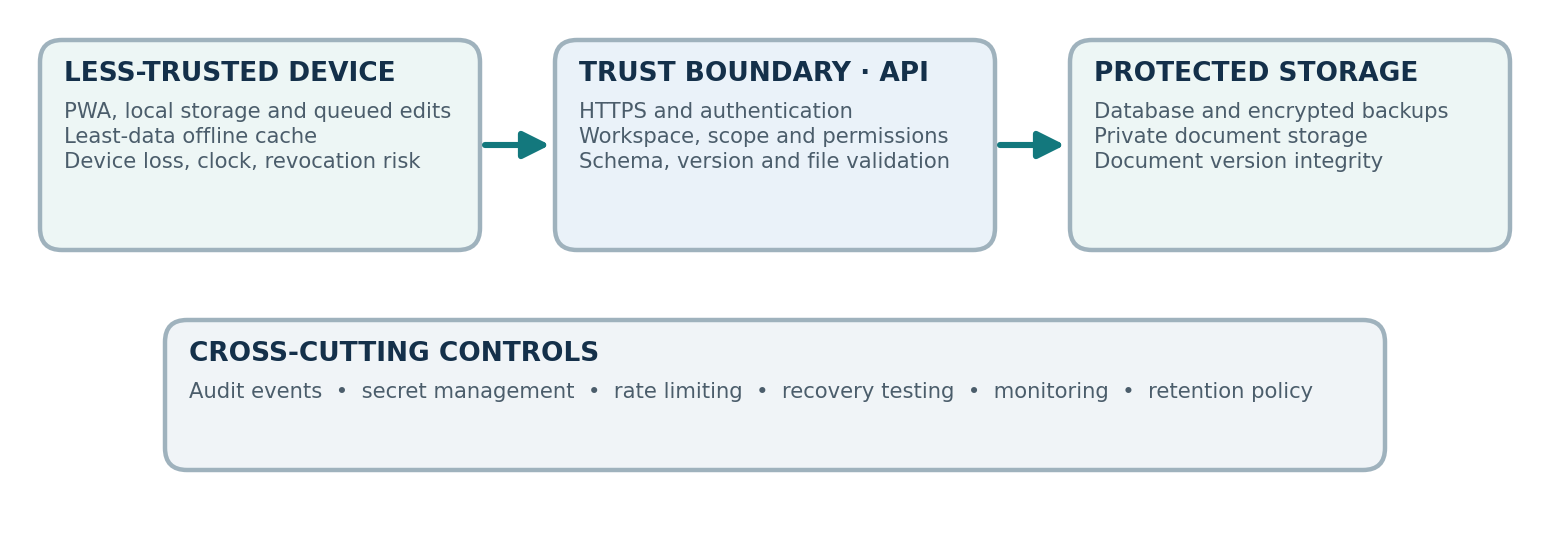
\includegraphics[width=\linewidth]{nfr-security-boundaries.png}
\caption{Proposed security boundaries and cross-cutting controls, adapted from the team's NFR contribution.}
\label{fig:nfr-security-boundaries}
\end{figure}

\Needspace{7\baselineskip}
\nfrheading{\identifier{SEC-01} --- Account authentication and password protection}\label{nfr:SEC-01}
The backend shall authenticate every application account using a unique, verified email identity and a password.

\textit{Rationale:} Protects the owner and included manager accounts against account takeover and enumeration.

\textit{Related:} \hyperref[fr:001]{\identifier{FR-001}}, \hyperref[fr:002]{\identifier{FR-002}}, \hyperref[fr:005]{\identifier{FR-005}}, \hyperref[fr:064]{\identifier{FR-064}}.
\begin{enumerate}[label=(\alph*),leftmargin=*,itemsep=1pt,topsep=3pt]
\item Only accounts with a verified email can access a business workspace; unverified accounts are refused.
\item Application-managed authentication uses established backend libraries and salted Argon2id password hashes; benchmark and record concrete cost parameters before deployment. Plaintext passwords are never stored or logged. A managed identity service is not the selected baseline.
\item Enforce at least 15 characters in the password-only flow and accept passphrases of at least 64 characters without silent truncation. Reject common/compromised passwords on registration, reset and change.
\item After five failed logins within 15 minutes, apply progressive throttling using account/source signals, without permanent attacker-triggered account lockout. Exact delay progression and recovery configuration require implementation review and tests.
\item Authentication failure responses do not disclose whether an email address is registered.
\end{enumerate}

\Needspace{7\baselineskip}
\nfrheading{\identifier{SEC-02} --- Online session lifecycle}\label{nfr:SEC-02}
Protected online requests shall use short-lived, revocable credentials.

\textit{Rationale:} Limits the exposure of stolen credentials and supports timely revocation.

\textit{Related:} \hyperref[fr:002]{\identifier{FR-002}}, \hyperref[fr:003]{\identifier{FR-003}}, \hyperref[fr:004]{\identifier{FR-004}}, \hyperref[fr:005]{\identifier{FR-005}}, \hyperref[fr:008]{\identifier{FR-008}}, \hyperref[fr:064]{\identifier{FR-064}}.
\begin{enumerate}[label=(\alph*),leftmargin=*,itemsep=1pt,topsep=3pt]
\item Online access credentials expire after 15 minutes; the server refuses expired credentials. Renewal is permitted only while the originating online session remains valid.
\item Renewable online sessions expire at most seven days after login, requiring authentication again; renewal does not extend that absolute limit. Implement revocation and rotation/replay protection. Cookie-based credentials use Secure, HttpOnly and an appropriate SameSite policy.
\item Logout revokes the applicable online session. Successful password reset or change invalidates existing online sessions. Membership revocation immediately denies that business online without deleting unrelated memberships.
\item An expired online session requires online renewal or authentication under its policy. It does not delete pending work or change the separate 15-day offline grant in \hyperref[nfr:AOC-02]{\identifier{AOC-02}}.
\end{enumerate}

\Needspace{7\baselineskip}
\nfrheading{\identifier{SEC-03} --- Workspace and operation-level authorisation}\label{nfr:SEC-03}
The server shall check authorisation on every protected read, write, export and file operation.

\textit{Rationale:} Preserves business isolation and independently granted consultation, entry and correction rights.

\textit{Related:} \hyperref[fr:002]{\identifier{FR-002}}, \hyperref[fr:004]{\identifier{FR-004}}, \hyperref[fr:007]{\identifier{FR-007}}, \hyperref[fr:008]{\identifier{FR-008}}, \hyperref[fr:023]{\identifier{FR-023}}, \hyperref[fr:038]{\identifier{FR-038}}, \hyperref[fr:053]{\identifier{FR-053}}; \hyperref[br:024]{\identifier{BR-024}}.
\begin{enumerate}[label=(\alph*),leftmargin=*,itemsep=1pt,topsep=3pt]
\item Each request validates account status and endpoint-specific authority. Technical provisioning requires the administrator system role; business operations require active workspace membership, responsibility scope and operation-specific grants. Administrator status alone grants no business-data/file authority.
\item A user-supplied identifier never establishes authority by itself.
\item Distinguish consultation, planning, entry, corrections, document association/modification, signing initiation and financial grants. Apply the included Field Manager defaults and mandatory scoped insurance access in Section~\ref{sec:permission-defaults}.
\item Supported financial actions may operate offline with the corresponding grants and prepared context; central acceptance revalidates them. Consultation/full-ticket access is disabled initially and requires an explicit owner grant within assigned scope; structured financial writes require additional grants.
\item Denied requests return a generic response that contains no protected data.
\end{enumerate}

\Needspace{7\baselineskip}
\nfrheading{\identifier{SEC-04} --- Encryption and private storage}\label{nfr:SEC-04}
Protected business data shall be encrypted in transit and in central storage; service credentials shall be protected and stored files private by default. Password storage follows \identifier{SEC-01} rather than reversible password encryption.

\textit{Rationale:} Protects employment, insurance and signing information across the device, API and storage boundaries.

\textit{Related:} \hyperref[fr:002]{\identifier{FR-002}}, \hyperref[fr:038]{\identifier{FR-038}}, \hyperref[fr:039]{\identifier{FR-039}}, \hyperref[fr:040]{\identifier{FR-040}}, \hyperref[fr:042]{\identifier{FR-042}}.
\begin{enumerate}[label=(\alph*),leftmargin=*,itemsep=1pt,topsep=3pt]
\item Production requests use HTTPS and a reviewed TLS/HSTS configuration. Plain HTTP is redirected or refused before protected content or credentials are served. The minimum supported protocol and deployment settings are reviewed under \decisionref{Q-TECH-01}.
\item Encrypt the central database, backups and private file storage at rest, with controlled key access and rotation. The hosting/key-management implementation is selected and verified during architecture review; this does not settle local-device protection under \decisionref{Q-DOC-07}.
\item Document storage is private by default; protected files are served only after API authorisation, using short-lived scoped retrieval links where applicable.
\item The central database is not directly reachable from the public internet.
\end{enumerate}

\Needspace{7\baselineskip}
\nfrheading{\identifier{SEC-05} --- Secure API, PWA and file validation}\label{nfr:SEC-05}
The backend shall validate every input and uploaded file independently of the PWA.

\textit{Rationale:} Prevents malicious requests, script injection and unsafe file handling; client-side validation does not replace server-side validation.

\textit{Related:} \hyperref[fr:001]{\identifier{FR-001}}, \hyperref[fr:038]{\identifier{FR-038}}, \hyperref[fr:040]{\identifier{FR-040}}, \hyperref[fr:045]{\identifier{FR-045}}, \hyperref[fr:049]{\identifier{FR-049}}, \hyperref[fr:051]{\identifier{FR-051}}, \hyperref[fr:053]{\identifier{FR-053}}, \hyperref[fr:063]{\identifier{FR-063}}, \hyperref[fr:064]{\identifier{FR-064}}.
\begin{enumerate}[label=(\alph*),leftmargin=*,itemsep=1pt,topsep=3pt]
\item Types, identifiers, relationships and file sizes are validated on the server, including references across business workspaces.
\item Use parameterised database access, context-appropriate output encoding, restrictive CORS and a deployable Content Security Policy. Cookie-authenticated state changes also require effective CSRF protection; CORS alone is not an authorisation or CSRF control.
\item Worker uploads accept PDF, JPG and PNG within the 10~MB (10,000,000-byte) per-file limit in \hyperref[br:044]{\identifier{BR-044}}. Validate content, size and safe file handling server-side, not only the extension. The team tests the 10,000,000-byte boundary and representative files under \decisionref{Q-DOC-06}; JPEG is accepted as the JPG image format.
\item Ticket, analysis and valuation evidence uses the same approved formats and 10~MB limit. Complete source files may be prepared offline with their consultation grants; monetary content neither forces classification/redaction nor prohibits upload under the applicable entry grant. Successful attachment replacement deletes its old file without history under \decisionref{Q-AT-02}; failed transfers preserve the old file and remain recoverable.
\item Scan application and bundled dependencies for known vulnerabilities in the delivery pipeline, triage findings and record remediation or explicit risk acceptance before release. A successful scan is not a claim of absence of vulnerabilities.
\end{enumerate}

\Needspace{7\baselineskip}
\nfrheading{\identifier{SEC-06} --- Secrets and deployment identities}\label{nfr:SEC-06}
Production credentials shall be kept out of source control and PWA assets, and every pipeline and service shall use least-privilege identities.

\textit{Rationale:} Prevents compromise through repository leakage or excessive pipeline privileges.

\textit{Related:} \hyperref[fr:001]{\identifier{FR-001}}, \hyperref[fr:005]{\identifier{FR-005}}, \hyperref[fr:040]{\identifier{FR-040}}.
\begin{enumerate}[label=(\alph*),leftmargin=*,itemsep=1pt,topsep=3pt]
\item Do not commit production service credentials or bundle database/email/storage secrets into the PWA. Device-local protection material, if used, follows the separate reviewed design under \decisionref{Q-DOC-07}.
\item Runtime services and delivery-pipeline jobs use separate identities with least privilege.
\item Keep production secrets in an access-controlled secrets mechanism with documented rotation and access review. Provider/tool selection remains an implementation decision.
\end{enumerate}

\Needspace{7\baselineskip}
\nfrheading{\identifier{SEC-07} --- Security-event audit logging}\label{nfr:SEC-07}
The server shall record security-relevant events.

\textit{Rationale:} Supports investigation and accountability while preserving the rule that ordinary business updates retain current values only (Section~\ref{sec:identity-current-values}).

\textit{Related:} \hyperref[fr:003]{\identifier{FR-003}}, \hyperref[fr:005]{\identifier{FR-005}}, \hyperref[fr:007]{\identifier{FR-007}}, \hyperref[fr:008]{\identifier{FR-008}}, \hyperref[fr:036]{\identifier{FR-036}}, \hyperref[fr:037]{\identifier{FR-037}}, \hyperref[fr:042]{\identifier{FR-042}}.
\begin{enumerate}[label=(\alph*),leftmargin=*,itemsep=1pt,topsep=3pt]
\item Each event records server timestamp, initiating account when known, workspace where applicable, action, minimal target identifier and outcome.
\item Mandatory server-observable categories: successful/failed authentication, logout, account recovery, membership and permission changes, restricted-document access requests handled by the API or controlled file service, signing acceptance, denied operations, revoked-access recovery decisions and security-relevant synchronisation conflicts. For document access, record the authorised retrieval/link-issuance decision or refusal; this does not prove that the user viewed the file.
\item Logs exclude passwords, raw tokens/full lifecycle links, document bodies, signature images, full official identification and raw monetary values; use minimal authorised identifiers.
\item Retain security events for 90 days from the server event, accessible only to authorised operations/investigation personnel. Purge thereafter, except justified incident preservation with a documented purpose and scope; test the configured schedule.
\item This requirement does not impose a permanent field-by-field history on ordinary corrections.
\item Opening a prepared file entirely offline is not logged in this version. Server preparation/retrieval/link issuance does not prove viewing. This coverage choice does not weaken file-access authorisation.
\end{enumerate}

\Needspace{7\baselineskip}
\nfrheading{\identifier{SEC-08} --- Document and signature integrity}\label{nfr:SEC-08}
Each accepted document version and each confirmed signature shall be tamper-evident and bound to the exact version signed.

\textit{Rationale:} Preserves integrity and provenance while respecting current-source replacement policy and withdrawal.

\textit{Related:} \hyperref[fr:038]{\identifier{FR-038}}, \hyperref[fr:041]{\identifier{FR-041}}, \hyperref[fr:042]{\identifier{FR-042}}, \hyperref[fr:043]{\identifier{FR-043}}, \hyperref[fr:044]{\identifier{FR-044}}, \hyperref[fr:045]{\identifier{FR-045}}; \hyperref[br:026]{\identifier{BR-026}}.
\begin{enumerate}[label=(\alph*),leftmargin=*,itemsep=1pt,topsep=3pt]
\item Each current accepted source has an immutable file identity and protected cryptographic digest. Verify source bytes against that digest. Validate the rendition against its own source/worker/signature associations; a derived PDF is not compared with the source digest. The team selects/tests the digest algorithm and metadata protection; a hash is not signer identification.
\item Bind a confirmed drawing to its worker, authorised initiator, exact source and confirmation time.
\item Never transfer a drawing or choice to another source/worker or overwrite signed bytes in place. A replacement needs its own worker review/signing.
\item Apply \identifier{BR-026}: only after successful replacement, delete the superseded source, signature and PDF, including signed contracts/externally declared signed uploads. Invalidate old-source signing and propagate received deletion to prepared copies. Temporary rejected-proposal recovery follows \decisionref{Q-DOC-04}, without a history browser.
\item Record server acceptance time separately from device confirmation time.
\item A drawn mark alone is not represented as a qualified electronic signature.
\end{enumerate}

\Needspace{7\baselineskip}
\nfrheading{\identifier{SEC-09} --- Verification, recovery and invitation tokens}\label{nfr:SEC-09}
Account-lifecycle links shall be single-use, short-lived and unpredictable.

\textit{Rationale:} Protects registration, recovery and invitation flows from replay, enumeration and unauthorised business membership.

\textit{Related:} \hyperref[fr:001]{\identifier{FR-001}}, \hyperref[fr:005]{\identifier{FR-005}}, \hyperref[fr:006]{\identifier{FR-006}}, \hyperref[fr:064]{\identifier{FR-064}}.
\begin{enumerate}[label=(\alph*),leftmargin=*,itemsep=1pt,topsep=3pt]
\item Owner-activation and email-verification links, including replacement-email verification, expire after 24 hours and are single-use. An unverified replacement cannot supersede the active email; a resend invalidates the preceding link.
\item Password-reset links expire after 30 minutes and are single-use. Resending invalidates the preceding link; invalid/expired/consumed links cannot change credentials.
\item Invitations expire after seven days and are single-use, bound to the intended verified email and business. Resending/cancelling invalidates superseded links without duplicate membership.
\item Generate token values unpredictably and store only a verification hash or equivalent protected verifier when persisted. Consume/invalidate lifecycle authorisations transactionally. Retries may report an already completed action without repeating activation, membership creation or credential changes.
\item A successful reset revokes existing online sessions without changing business ownership.
\end{enumerate}

\Needspace{7\baselineskip}
\nfrheading{\identifier{SEC-10} --- Abuse protection and rate limiting}\label{nfr:SEC-10}
The API shall limit request rates to protect availability and prevent automated abuse.

\textit{Rationale:} \hyperref[nfr:SEC-01]{\identifier{SEC-01}} throttles login attempts only; recovery, invitation, upload and email-triggering endpoints can also be abused.

\textit{Related:} \hyperref[fr:001]{\identifier{FR-001}}, \hyperref[fr:005]{\identifier{FR-005}}, \hyperref[fr:006]{\identifier{FR-006}}, \hyperref[fr:040]{\identifier{FR-040}}.
\begin{enumerate}[label=(\alph*),leftmargin=*,itemsep=1pt,topsep=3pt]
\item Use account/source/recipient-aware limits as applicable: unauthenticated operations cannot depend on an authenticated account key. Apply stricter reviewed controls to authentication, recovery, invitations, uploads and email-triggering requests.
\item Exceeded limits return a generic, retryable rejection and do not affect other accounts.
\item Resending verification, reset and invitation messages is limited per recipient address.
\item The approved login threshold is five failures within 15 minutes under SEC-01. Endpoint-specific recovery, resend, upload and invitation limits and progressive delays still require configuration review; verify recipient/account isolation before release.
\end{enumerate}

\Needspace{7\baselineskip}
\nfrheading{\identifier{SEC-11} --- Email delivery security}\label{nfr:SEC-11}
Verification, recovery and invitation messages shall be sent through an authenticated and monitored email delivery service.

\textit{Rationale:} Protects account activation, recovery, verified-email changes and invitations that depend on email delivery.

\textit{Related:} \hyperref[fr:001]{\identifier{FR-001}}, \hyperref[fr:005]{\identifier{FR-005}}, \hyperref[fr:006]{\identifier{FR-006}}, \hyperref[fr:064]{\identifier{FR-064}}.
\begin{enumerate}[label=(\alph*),leftmargin=*,itemsep=1pt,topsep=3pt]
\item The sending domain is authenticated with SPF, DKIM and DMARC.
\item Messages contain the intended lifecycle link and minimal account context, never passwords, worker data or protected documents.
\item A send failure preserves the pending account/invitation state without duplicate identities or memberships. Offer rate-limited resend, invalidating the preceding lifecycle link. Recovery acknowledgements remain generic regardless of registration status.
\item Record the provider, its processing role/terms, sending-domain configuration and any transfers in the processing inventory under \hyperref[nfr:PRV-05]{\identifier{PRV-05}}; provider selection remains under \decisionref{Q-NFR-05}.
\end{enumerate}

\paragraph{Email delivery operation.}
Only the backend calls the transactional email service using protected credentials.
Record technical send outcomes and provider failures without full links. Provider
acceptance does not prove inbox delivery or reading. Development/demo sending uses
controlled recipients or a test environment. Provider, authorised sender domain and
concrete configuration remain under \decisionref{Q-NFR-05}.

\paragraph{Technical references.}
Password and session controls are informed by the
\href{https://cheatsheetseries.owasp.org/cheatsheets/Authentication_Cheat_Sheet.html}{OWASP Authentication},
\href{https://cheatsheetseries.owasp.org/cheatsheets/Password_Storage_Cheat_Sheet.html}{Password Storage}
and \href{https://cheatsheetseries.owasp.org/cheatsheets/Session_Management_Cheat_Sheet.html}{Session Management}
guidance. These references do not approve project-specific numeric targets.

\paragraph{Administrator provisioning verification.}
Check administrator-only owner setup, single-client concurrency/idempotency,
expired/replayed activation, controlled resend and recipient-chosen password.
Unauthenticated users, owners and managers cannot call technical provisioning;
technical administrators cannot read agricultural records/files by system role alone.
Manager signup requires an intended valid owner invitation. Bootstrap credentials
are deployment-managed; passwords never enter provisioning messages or logs.
